%--------------------------------------------------------
%--------------------------------------------------------
\comment{How does the radial kernel reduce to unity on evaluating the the operator on to its inverse ? This will be important to understand how to define alternate radial functions.}
\section{Generalized operators}
The azimuthal dependence of the convolution kernels which translate the Stokes parameters Q \& U to the scalar E \& B is determined by the spin properties of the field being operated upon and the spin of the resultant fields. Hence there is no freedom in the choice of function for the azimuthal dependence of the convolution kernels. The radial part of the function however is determined by the choice of the basis functions.  It is possible to generalize these convolution kernels by choosing alternate forms for the radial functions.

We can characterize different forms of the radial kernel by introducing the following harmonic space operator,
%
\beq
\tilde{\mathcal{G}} = {\begin{bmatrix} b_{\ell}^E & 0  \\  0 & b_{\ell}^B \end{bmatrix}} \,,
\eeq
%
where the functions $b^E_{\ell}$ and $b^B_{\ell}$ represent the harmonic representation of the modified radial functions and can in the most general case be chosen to be different for E and B modes. To simplify the discussion and without loosing this generality we proceed with the assumption $b_{\ell}^E = b_{\ell}^B= b_{\ell}$. We can chose this function to be any arbitrary function and it will allow us to define some convolution operator which either translates Stokes Q \& U parameters to scalars E \& B or vice verse. Given $\tilde{\mathcal{G}}$ the modified forward and inverse convolution kernels are given by the following expressions,
%
\begin{subequations} \label{eq:gen_qu2eb}
\beqry
{\bar O}' &=& {{}_0\mathcal{Y}} *\tilde T^{-1}*\tilde{\mathcal{G}}* {{}_2\mathcal{Y}^{\dagger}} *\bar T \,,\\
{\bar O}'^{-1}&=& \bar{T}^{-1} *{{}_2\mathcal{Y}}* \tilde{\mathcal{G}}^{-1} *\tilde T *{{}_0\mathcal{Y}^{\dagger}}
\eeqry
\end{subequations}
%
where we have used the primed notation  to distinguish these generalized operators from the default operators defined in \sec{sec:qu2eb} and \sec{sec:eb2qu}. Note that for an arbitrary choice of $\tilde{\mathcal{G}}$ only one of the operators in \eq{eq:gen_qu2eb} is well defined, since $\tilde{\mathcal{G}}^{-1}$ may be ill defined. If we require both the forward and inverse hold true, then we are constrained in choosing $\tilde{\mathcal{G}}$ such that its inverse is well defined.

The radial part of the convolution kernel which translates Stokes parameters Q \& U to scalar E \& B is given by the following expression,
%
\beq
R_{QU \leftrightarrow EB}(\beta) = R(\beta) = \sum _{\ell=\ell_{\rm min}} ^{\ell_{\rm max}}\sqrt{\frac{2 \ell+1}{4 \pi} \frac{(\ell-2)!}{(\ell + 2)!}} P_{\ell}^2(\cos{\beta}) \,,\label{eq:native_rad}
\eeq
%
where $P_{\ell}^{2}$ are the associated Legendre polynomials. Note that the form of the radial kernel remains unchanged for the forward $\bar{O}$ and the inverse operators $\bar{O}^{-1}$. 

While translating from Stokes Q \& U parameters which form a spin-2 field to spin-0 scalars E \& B, the azimuthal part of the convolution is restricted to have the form $e^{-i2\phi}$. The only freedom is to choose the radial part of the convolution kernel.  It is possible to generalize the form of the radial kernel by introducing the following redefinition,
%
\beq
G_{QU \rightarrow EB}(\beta) = G(\beta) = \sum _{\ell=\ell_{\rm min}} ^{\ell_{\rm max}} b_{\ell}\sqrt{\frac{2 \ell+1}{4 \pi} \frac{(\ell-2)!}{(\ell + 2)!}} P_{\ell}^2(\cos{\beta}) \,,\label{eq:mod_rad_forward}
\eeq
%
where $b_{\ell}$ encodes the desired changes to the radial function. This radial function now defines the modified forward operator $\bar{O}'$. Since we require the following property: $\bar{O}' \bar{O}'^{-1} = I$ to hold true, the inverse operator cannot have the same form for the radial function. Demanding $\bar{O}' \bar{O}'^{-1} = I$ to hold true it can be shown that the modified operator and its inverse is given by the following equations,
%
\begin{subequations}
\beqry
{\bar O} &=& {{}_0\mathcal{Y}} *\tilde T^{-1}*\tilde{\mathcal{G}}* {{}_2\mathcal{Y}^{\dagger}} *\bar T \,,\\
{\bar O}^{-1}&=& \bar{T}^{-1} *{{}_2\mathcal{Y}}* \tilde{\mathcal{G}}^{-1} *\tilde T *{{}_0\mathcal{Y}^{\dagger}}
\eeqry
\end{subequations}
%
where it can be shown that the radial part of the inverse operator has to take up the following form,
%
\beq
G_{EB \rightarrow QU}(\beta) = G^{-1}(\beta) = \sum _{\ell=\ell_{\rm min}} ^{\ell_{\rm max}} b_{\ell}^{-1}\sqrt{\frac{2 \ell+1}{4 \pi} \frac{(\ell-2)!}{(\ell + 2)!}} P_{\ell}^2(\cos{\beta}) \,,\label{eq:mod_rad_inverse}
\eeq
%
where $b_{\ell}$ is the same multipole function introduced in \eq{eq:mod_rad_forward}. Therefore for the forward and backward operators to be well behaved we are restricted in choosing multipole functions $b_{\ell}$ such that its inverse is well defined. If this constraint is overlooked, the ability to transform back and forth between the Stokes parameters and the scalar representation of the CMB polarization field is compromised. Given this general definition for the radial function $G(\beta)$, note that the radial function $R(\beta)$ is just a special case formed by making the choice $b_{\ell}=1$. Note that for this choice the inverse of the multipole function is itself $b_{\ell}^{-1} = b_{\ell}$ and therefore $G^{-1}(\beta) = G(\beta)$.

While modifying the radial function, it makes more sense to make a choice on the real space function $G(\beta)$ instead of choosing the multipole function $b_{\ell}$. We use the orthogonality property of associated Legendre polynomials to express the multipole function $b_{\ell}$ as,
%
\beq
b_{\ell} = 2 \pi \sqrt{\frac{(\ell-2)!}{(\ell+2)!}} \int _{0}^{\pi} G(\beta) P_{\ell}^{2}(\cos{\beta}) d\cos{\beta} \,, \label{eq:gb2bl}
\eeq
%
where we have used the orthonormality property of the associated Legendre polynomials to arrive at the above equation. Note that once the choice of $G(\beta)$ is made, the inverse function $G^{-1}(\beta)$ is automatically defined by the forward relation given in \eq{eq:mod_rad_inverse}.

In \sec{sec:local_conv_eb} we constructed localized convolution kernels by multiplying $R(\beta)$ with an apodized version of the step function $\theta_{\rm apo}(r_{\rm cutoff})$. The oscillation seen in the spectra in \fig{fig:eb-spectra_rad_cutoff} can be explained to be due to this effective beam characterized by $b_{\ell}^2$ operating on the power spectra. The effective beam can be evaluated by computing the multipole function $b_{\ell}$ as follows,
%
\beq
b_{\ell} = 2 \pi \sqrt{\frac{(\ell-2)!}{(\ell+2)!}} \int _{0}^{r_{\rm cutoff}} R(\beta) \theta_{\rm apo}(r_{\rm cutoff})  P_{\ell}^{2}(\cos{\beta}) d\cos{\beta} \,, \label{eq:gb2bl} \,,
\eeq
%
where the upper limit of the integration is set to $r_{\rm cutoff}$ since the function $\theta_{\rm apo}(r_{\rm cutoff})$ vanishes for $\beta>r_{\rm cutoff}$. The function $b^2_{\ell}-1$ matches the oscillation seen in \fig{fig:eb-spectra_rad_cutoff} as  seen in \fig{fig:match_cl_oscillations} where the two results have been over plotted.
%
\begin{figure}[!t] 
\centering
\subfigure[]{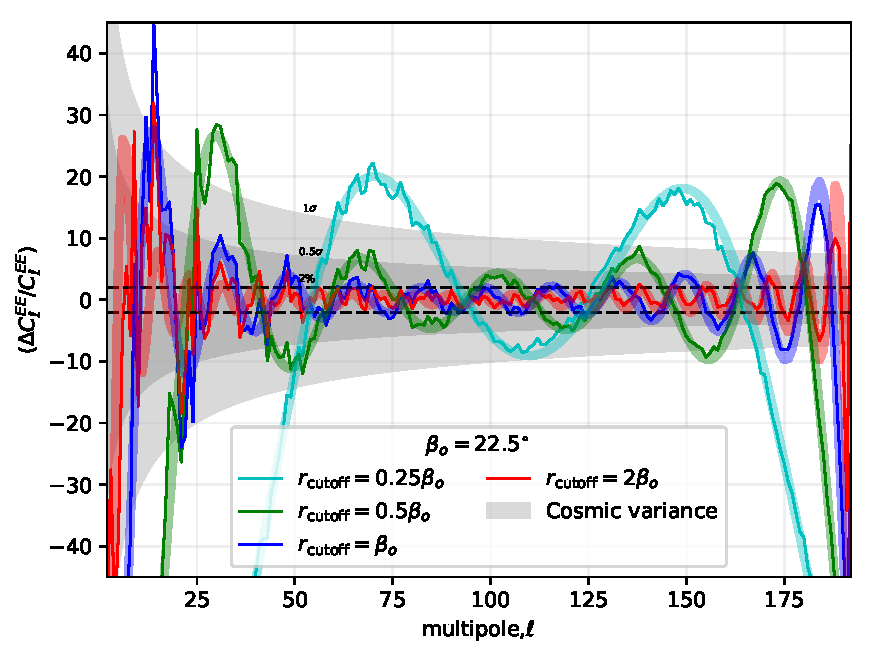
\includegraphics[width=0.98\columnwidth]{analytical_cl_oscillations_vs_data.pdf}}
\caption{The thin lines depicts the same spectral differences as those seen in \fig{fig:eb-spectra_rad_cutoff}, while the thick lines of the corresponding color depict the function $b_{\ell}^2 -1$ as derived from evaluating \eq{eq:gb2bl} for different $r_{\rm cutoff}$}.
\label{fig:match_cl_oscillations}
\end{figure}
%
The apodized step function in this case transition from 1 at $\beta < r_{\rm cutoff} -w$ to 0 at $r_{\rm cutoff}$ over a width $w= 3^{\circ}$ with a cosine squared profile .

%
\begin{figure}[!t] 
\centering
\subfigure[]{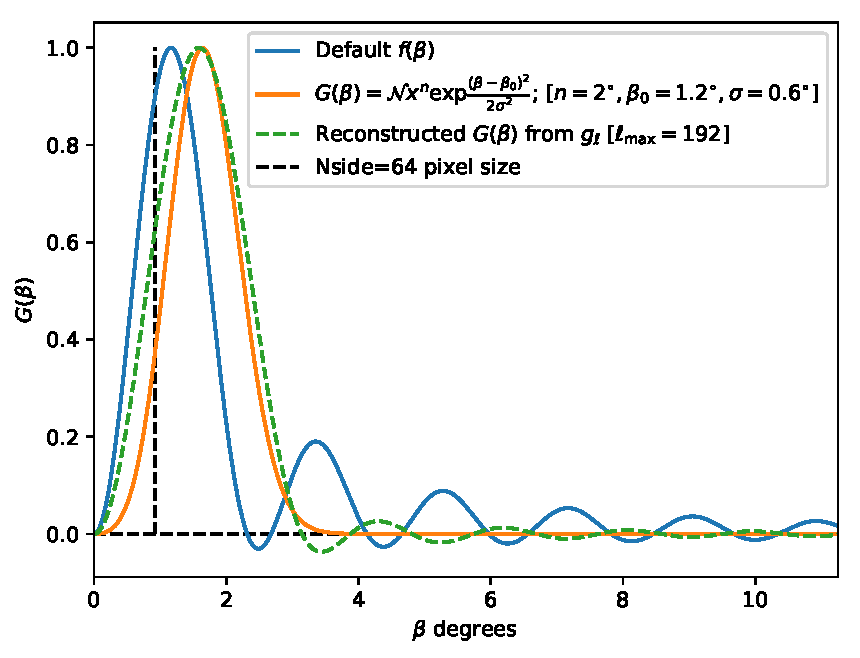
\includegraphics[width=0.49\columnwidth]{example_gbeta.pdf}}
\subfigure[]{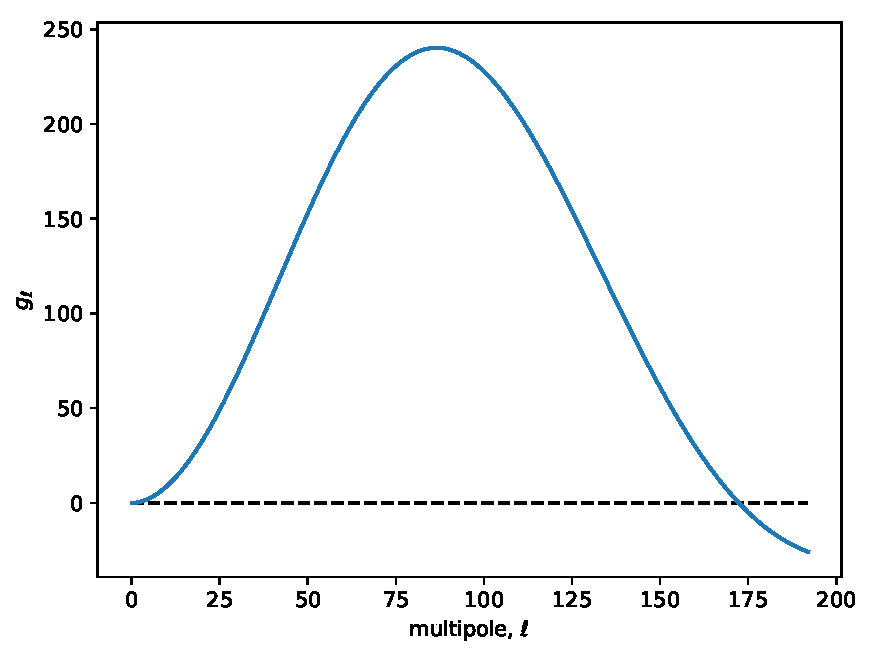
\includegraphics[width=0.49\columnwidth]{example_eff_bl.pdf}}
\caption{}
\label{fig:example_gbeta}
\end{figure}
%
%--------------------------------------------------------
%--------------------------------------------------------
